\documentclass[a4paper,11pt]{article}
\usepackage[left=0.85in,right=0.85in,top=0.80in,bottom=0.80in]{geometry}
\usepackage{listings}
\usepackage{amsmath}
\usepackage{fmtcount}
\usepackage{datetime}
\usepackage[pdftex]{graphicx}
\usepackage{fancyhdr}
\usepackage{color}
\usepackage{fancyvrb}
\usepackage{tabu}
\usepackage{xcolor}\newcommand{\squeezeup}{\vspace{-7mm}}
\begin{document}
\begin{center}
{\Huge Problem ID: zamboni}\vspace{2 mm} \\	% Problem Letter
{\huge Smoothing Ice}\vspace{2 mm} \\	% Problem Name
\end{center}
\setcounter{page}{15}
\large{
An ice resurfacer (also known as a \emph{Zamboni}) is a vehicle used to create a smooth layer of ice in an ice rink. We will model an ice rink as a two-dimensional grid with $N$ rows and $M$ columns (where the top-left most position is designated as $(0, 0)$ and the bottom-right most position is $(N-1, M-1)$). Each spot on the grid represents a patch of ice in the ice rink; a patch can be either \emph{rough} or \emph{smooth}. Initially each patch of ice is rough.\\\\
The Zamboni wants to clean the ice as fast as possible, but exactly how long will it take? Initially, the Zamboni starts on position $(x, y)$ facing north. Whenever the Zamboni is on top of a patch of ice, the ice gets smoothed. The Zamboni follows a very regular pattern to clean the ice; at each step, the Zamboni moves $t$ times in its current direction (initially $t=1$), turns 90 degrees clockwise, and then increments $t$ (that is, the next step the Zamboni will move over $t+1$ patches of ice). \emph{Note: a step is defined as the whole process of moving $t$ steps, changing direction, and incrementing the counter. Namely, the Zamboni may move over multiple patches of ice in the same step!} There's one more catch, however... the grid wraps around! If the Zamboni moves off an edge, it emerges on the opposite side of the grid. The figures below show the steps that the Zamboni must go through to clean a 2x2 grid starting at position $(0,0)$.
\begin{figure}[!htb]
\minipage{0.32\textwidth}
  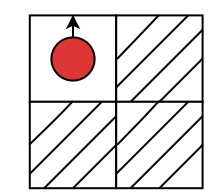
\includegraphics[width=\linewidth]{step1pt1.png}
  \caption{Initially the Zamboni faces upward.}\label{fig:awesome_image1}
\endminipage\hfill
\minipage{0.32\textwidth}
  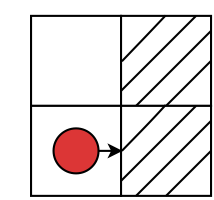
\includegraphics[width=\linewidth]{step2pt1.png}
  \caption{This is the configuration after step one.}\label{fig:awesome_image2}
\endminipage\hfill
\minipage{0.32\textwidth}%
  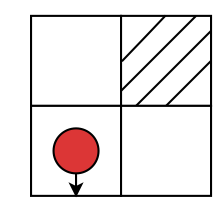
\includegraphics[width=\linewidth]{step3pt1.png}
  \caption{This is the configuration after step two.}\label{fig:awesome_image3}
\endminipage
\end{figure}
\begin{figure}[!htb]
\center
\minipage{0.32\textwidth}
  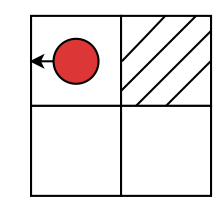
\includegraphics[width=\linewidth]{step4pt1.png}
  \caption{This is the configuration after step three.}\label{fig:awesome_image2}
\endminipage\hfill
\minipage{0.32\textwidth}%
  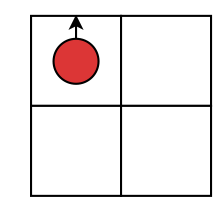
\includegraphics[width=\linewidth]{step4end.png}
  \caption{This is the configuration after step four.}\label{fig:awesome_image3}
\endminipage
\end{figure}

\newpage
\noindent
Given the size of the ice rink and the starting position of the Zamboni, can you determine how many steps it will take to smooth all of the ice in the rink?
}
\vspace{7mm}\\
\large{\bf{Input}}\vspace{2mm}\\
The input will begin with a line containing a single positive integer, $t$, representing the number of test cases to process. Each test case will consist of the four space separated integers $N$, $M$, $x$, and $y$ ($1 \leq N, M \leq 100$, $0 \leq x < N$, $0 \leq y < M$), each of which has the same meaning as defined above.
\vspace{3mm}\\
\large{\bf{Output}}\vspace{2mm}\\
For each test case print (on its own line) the number of steps it takes for the Zamboni to finish cleaning the ice.
\vspace{5mm}\\
\bf{Sample Input} \hspace{52mm} \bf{Sample Output}\vspace{1mm}\\
\begin{tabu*} to 475pt {|X[0r]|X[0l]|}
\tabucline-
\vspace{-\baselineskip} %needs to be placed here
\begin{Verbatim}
4
2 2 0 0
55 55 37 37
100 100 0 0
1 1 0 0
\end{Verbatim}
&
\vspace{-\baselineskip} %needs to be placed here
\begin{Verbatim}
4
164
298
0
\end{Verbatim}
\\
\tabucline-
\end{tabu*}
\end{document}
